\documentclass[11pt, a4paper]{article}
\usepackage{graphicx}
\usepackage{amsmath}
\usepackage{listings}
\usepackage{url}
\usepackage{geometry}

\usepackage{multicol}

\geometry{
 a4paper,
 total={170mm,257mm},
 left=20mm,
 top=20mm,
 }

\title{Assignment 4: Fourier Approximations} % Title

\author{JINEETH N [EE20B051]} % Author name

\date{\today} % Date for the report
\begin{document}	
		
\maketitle % Insert the title, author and date
\section*{Abstract}
%Create new section;it is autonumbered
\begin{itemize}
\item Fit two functions $e^{x}$ and $cos(cos(x))$ using the Fourier series coefficients calculated by least squares fitting method.
\item To plot graphs for better understanding
\end{itemize}


\section{Introduction}
The fourier function of a function $f(x)$ with period $2 \pi$ can be calculated as follows
\begin{equation}
    f(x) =  a_{0} + \sum\limits_{n=1}^{\infty} {{a_{n}\cos(nx)+b_{n}\sin(nx)}}
\end{equation}
where
\begin{equation}
         a_{0} = \frac{1}{2\pi}\int\limits_{0}^{2\pi} f(x)dx 
    \end{equation}
    \begin{equation}
         a_{n} = \frac{1}{\pi}\int\limits_{0}^{2\pi} f(x)\cos(nx)dx 
    \end{equation}
    \begin{equation}
         b_{n} = \frac{1}{\pi}\int\limits_{0}^{2\pi} f(x)\sin(nx)dx 
    \end{equation}

% \newpage
\section{Asssignment Tasks}
\subsection{Defining functions and plotting them}
\begin{verbatim}
    def expo(x):
    return exp(x)

    def coscos(x):
    pass
    return cos(cos(x))
        
    x = np.linspace(-2 * pi, 4 * pi, 1200)
    
    plt.semilogy(x, y_exp, label="True")
    plt.plot(xl[::5], yl_coscos[::5], "og", label="Predicted")
    

\end{verbatim}

\begin{figure}[!tbh]
   	\centering
   	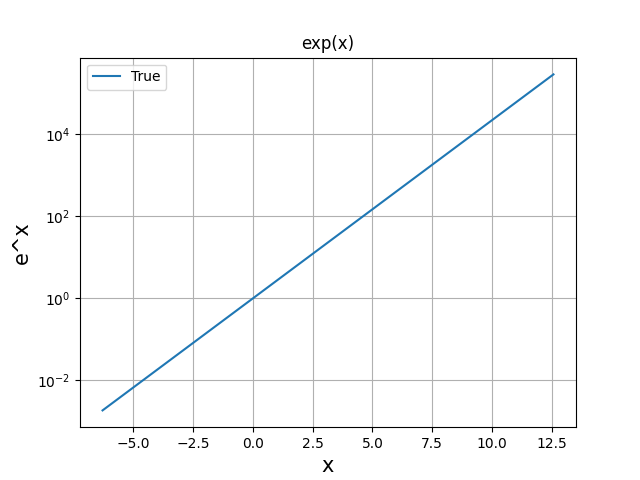
\includegraphics[scale=0.6]{Figure_1 1.png}   
   	\caption{Plotting $exp(x)$ in semilog scale}
   	\label{fig:sample}
   \end{figure} 
\begin{figure}[!tbh]
   	\centering
   	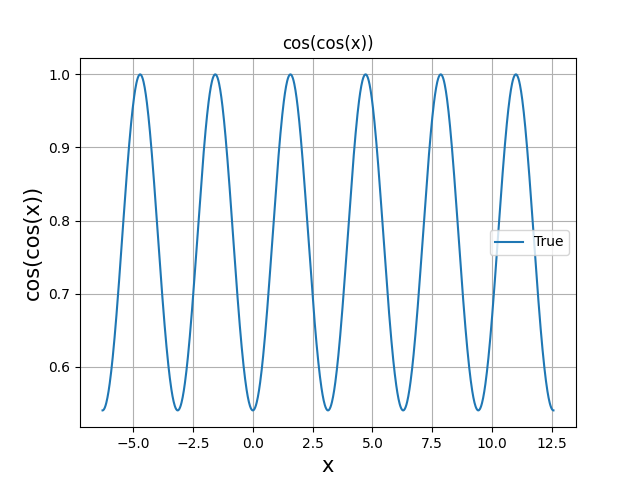
\includegraphics[scale=0.6]{Figure_2 1.png}   
   	\caption{Plotting $cos(cos(x))$ in semilog scale}
   	\label{fig:sample}
   \end{figure}
 
 \newpage
The plots for $cos(cos(x))$ and $exp(x)$ are shown above
\newpage
\subsection{Computing fourier coefficients using integration}
The first 51 coefficients are generated using the scipy.integrate.quad and the
equations mentioned in the introduction function.They are saved in the following
form
\begin{bmatrix}
           a_{0} \\
           a_{1} \\
           b_{1} \\
           \vdots \\
           a_{25} \\
           b_{25}
         \end{bmatrix}
\begin{verbatim}

       
    for k in range(26):

        
        if k != 0:
            c_coscos[p] = integrate.quad(a_coscos, 0, 2 * pi, args=(k))[0] / pi
            c_coscos[p + 1] = integrate.quad(b_coscos, 0, 2 * pi, args=(k))[0] / pi
            
            c_exp[p] = integrate.quad(a_exp, 0, 2 * pi, args=(k))[0] / pi
            c_exp[p + 1] = integrate.quad(b_exp, 0, 2 * pi, args=(k))[0] / pi
            p = p + 2

        
        else:
            c_coscos[p] = (integrate.quad(a_coscos, 0, 2 * pi, args=(k))[0] / pi) / 2
            c_exp[p] = (integrate.quad(a_exp, 0, 2 * pi, args=(k))[0] / pi) / 2
            p = p + 1
            
\end{verbatim}

\begin{itemize}
    \item Fourier coefficients of an even function should be zero. As expected $b_n$ is close to zero for $cos(cos(x))$ as it is an even function.
    \item The coefficients in a fourier series represent what are the frequencies happen to be in the output. The function cos(cos(x)) doesn't contain many different frequencies, so the values decay out quickly whereas the the exponential function is combination of different frequencies 
    \item The loglog plot is linear for $e^t$ because Fourier coefficients of $e^t$ decay with $1/n$ or $1/n^2$. The semilog plot is linear in $cos(cos(t))$ as the Fourier coefficients decay exponentially with n
\end{itemize}

\begin{figure}
  \centering
  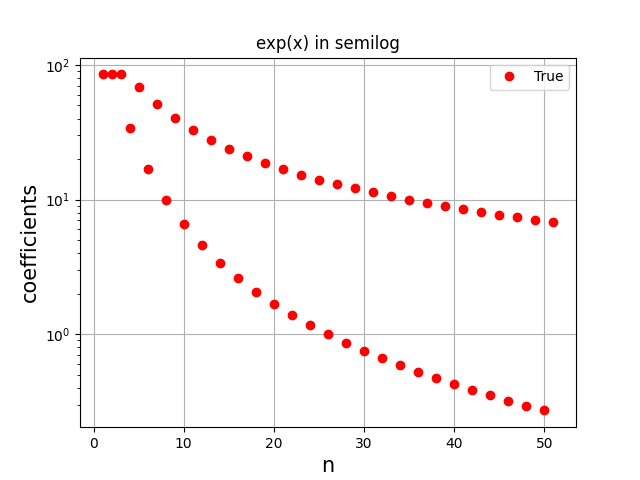
\includegraphics[scale=0.5]{Figure_3 1.png}
  \caption{semilog scale}
  \label{fig:sample}
 \end{figure}
 
\begin{figure}
  \centering
  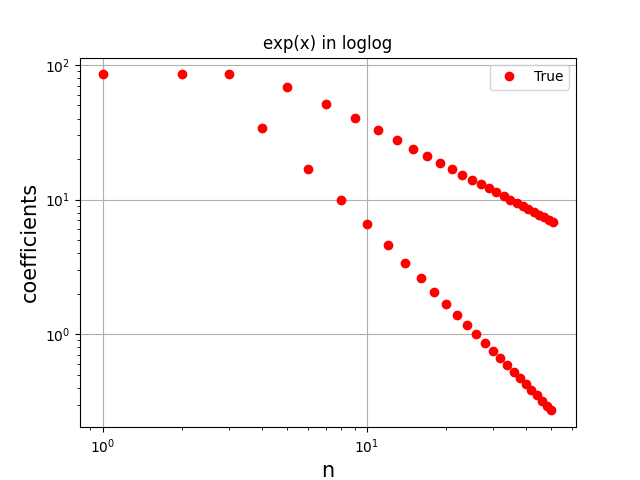
\includegraphics[scale=0.5]{Figure_4 1.png}
  \caption{loglog scale}
  \label{fig:sample}
\end{figure}

\begin{figure}
  \centering
  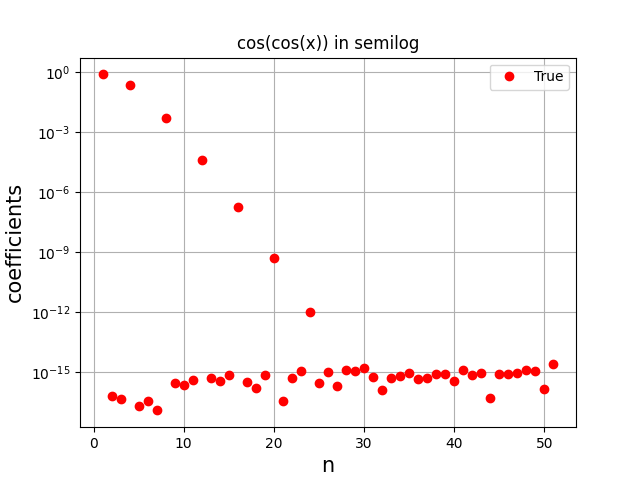
\includegraphics[scale=0.5]{Figure_5 1.png}
  \caption{semilog scale}
  \label{fig:sample}
\end{figure}

\begin{figure}
  \centering
  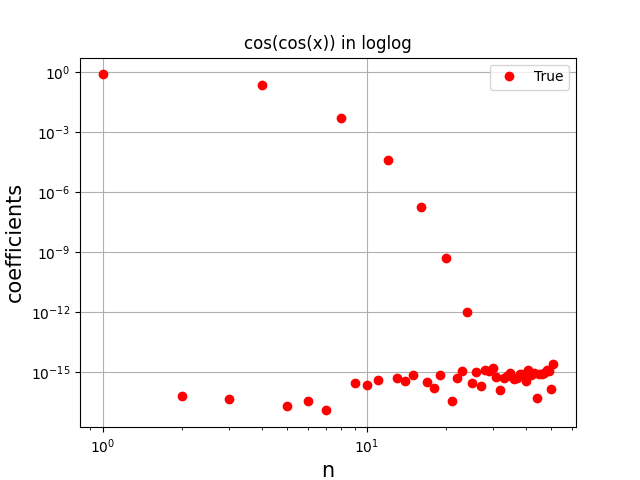
\includegraphics[scale=0.5]{Figure_6 1.png}
  \caption{loglog scale}
  \label{fig:sample}
\end{figure}

 \subsection{Using Least squares approach}
 Now, we used Least Squares approach to find the Fourier series coefficients. We linearly choose 400 x values in the range [0, 2$\pi$) and calculated coefficients using scipy.lstsq function
\begin{verbatim}

    A = np.zeros((400, 51))
A[:, 0] = 1
for k in range(1, 26):
    A[:, 2 * k] = sin(k * xl)
    A[:, 2 * k - 1] = cos(k * xl)
    
cl_exp = lstsq(A, B_exp, rcond=None)[0].reshape((-1, 1))
cl_coscos = lstsq(A, B_coscos, rcond=None)[0].reshape((-1, 1))

\end{verbatim}

\begin{figure}
  \centering
  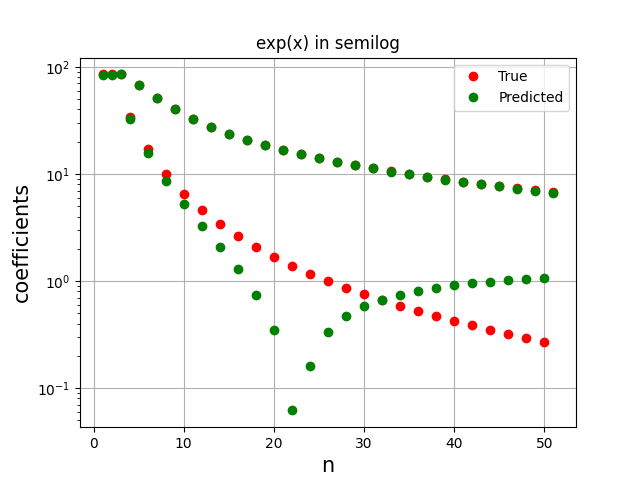
\includegraphics[scale=0.5]{Figure_3.png}
  \caption{semilogy scale}
  \label{fig:sample}
 \end{figure}

\begin{figure}
  \centering
  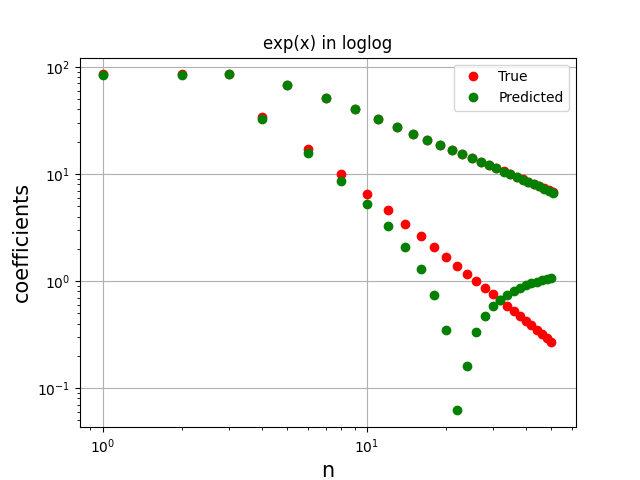
\includegraphics[scale=0.5]{Figure_4.png}
  \caption{loglogy scale}
  \label{fig:sample}
\end{figure}

\begin{figure}
  \centering
  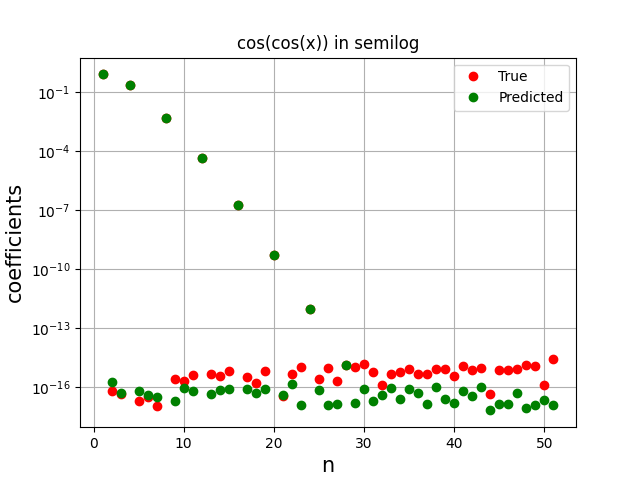
\includegraphics[scale=0.5]{Figure_5.png}
  \caption{semilogy scale}
  \label{fig:sample}
\end{figure}

\begin{figure}
  \centering
  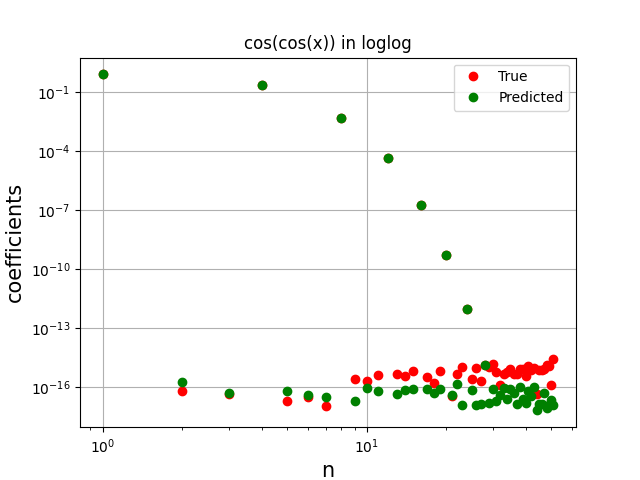
\includegraphics[scale=0.5]{Figure_6.png}
  \caption{loglogy scale}
  \label{fig:sample}
\end{figure}

The numpy linalg lstsq() solves the equation ax = b by computing a vector x that minimizes the Euclidean 2-norm $| b – ax |^2$
\begin{itemize}
    \item Maximum deviation  for $exp(x)$ is 1.3327 
    \item Maximum deviation  for $cos(cos(x))$ is 2.618e-15 
\end{itemize}
    We can observe error in $exp(x)$ $>>$ $cos(cos(x))$



\subsection{Plotting result}
The deviation in more in $exp(x)$ fitting beacuse fourier series exists only for periodic functions but $e^x$ is a non periodic function
\begin{figure}[!tbh]
   	\centering
   	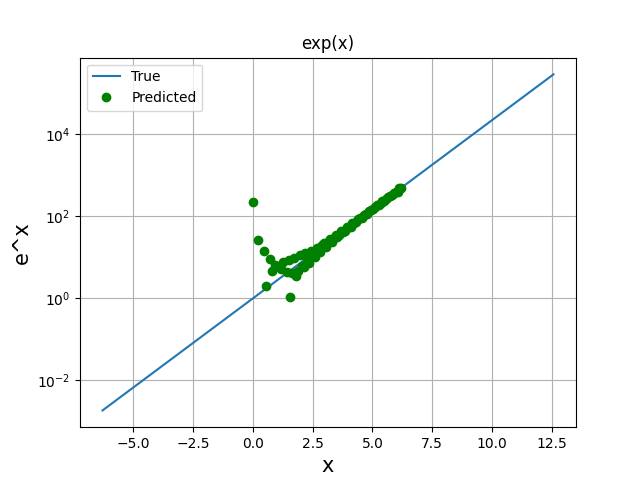
\includegraphics[scale=0.6]{Figure_1.png}   
   	\caption{Actual and predicted values of $exp(x)$}
   	\label{fig:sample}
   \end{figure}
   
   \begin{figure}[!tbh]
   	\centering
   	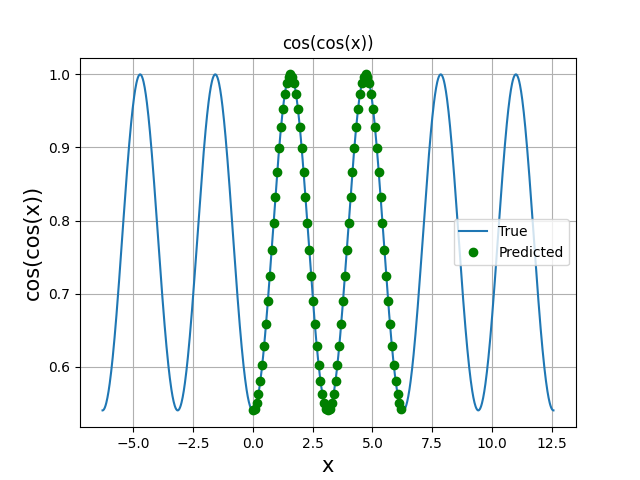
\includegraphics[scale=0.6]{Figure_2.png}   
   	\caption{Actual and predicted values of $cos(cos(x))$}
   	\label{fig:sample}
   \end{figure}
 
 \newpage
 \section{Conclusion}
    We computed Fourier series coefficients using two different methods
    \begin{itemize}
        \item Using integration
        \item Least Square Fitting method
    \end{itemize}
    We found close matching in two methods in case of $cos(cos(x))$ while, there
is a larger discrepancy in $exp(x)$
\end{document}